\documentclass[11pt]{article}

\usepackage[margin=1in]{geometry}
\usepackage{amsmath,amssymb,amsthm,mathrsfs}
\usepackage{graphicx}
\usepackage[hidelinks]{hyperref}

\newtheorem{theorem}{Theorem}
\newtheorem{lemma}{Lemma}

\newcommand{\F}{\mathscr F}
\newcommand{\BAP}{\mathrm{BAP}}
\newcommand{\Lip}{\operatorname{Lip}}
\newcommand{\Id}{\operatorname{Id}}
\newcommand{\norm}[1]{\left\lVert #1\right\rVert}

\title{A Free-Space Pair Counterexample for BAP of Banach Pairs}
\author{fa\_banach\_001, agent\_lane\_12}
\date{2026-06-20}

\begin{document}
\maketitle

\section*{Status}

This packet gives a likely valid counterexample to one natural reading of the
Section 7 question in Chavez-Dominguez, \emph{An Ando-Choi-Effros lifting
theorem respecting subspaces}, arXiv:1702.04774. For Banach-space pairs, BAP
of the Lipschitz-free pair \((\F(X),\F(Y))\) does not imply BAP of the original
pair \((X,Y)\).

\section*{Source Passage}

The source first gives a separable pair with Lipschitz BAP but not BAP, and
then asks whether an analogue of the Godefroy-Kalton free-space result holds
for pairs:

\begin{center}
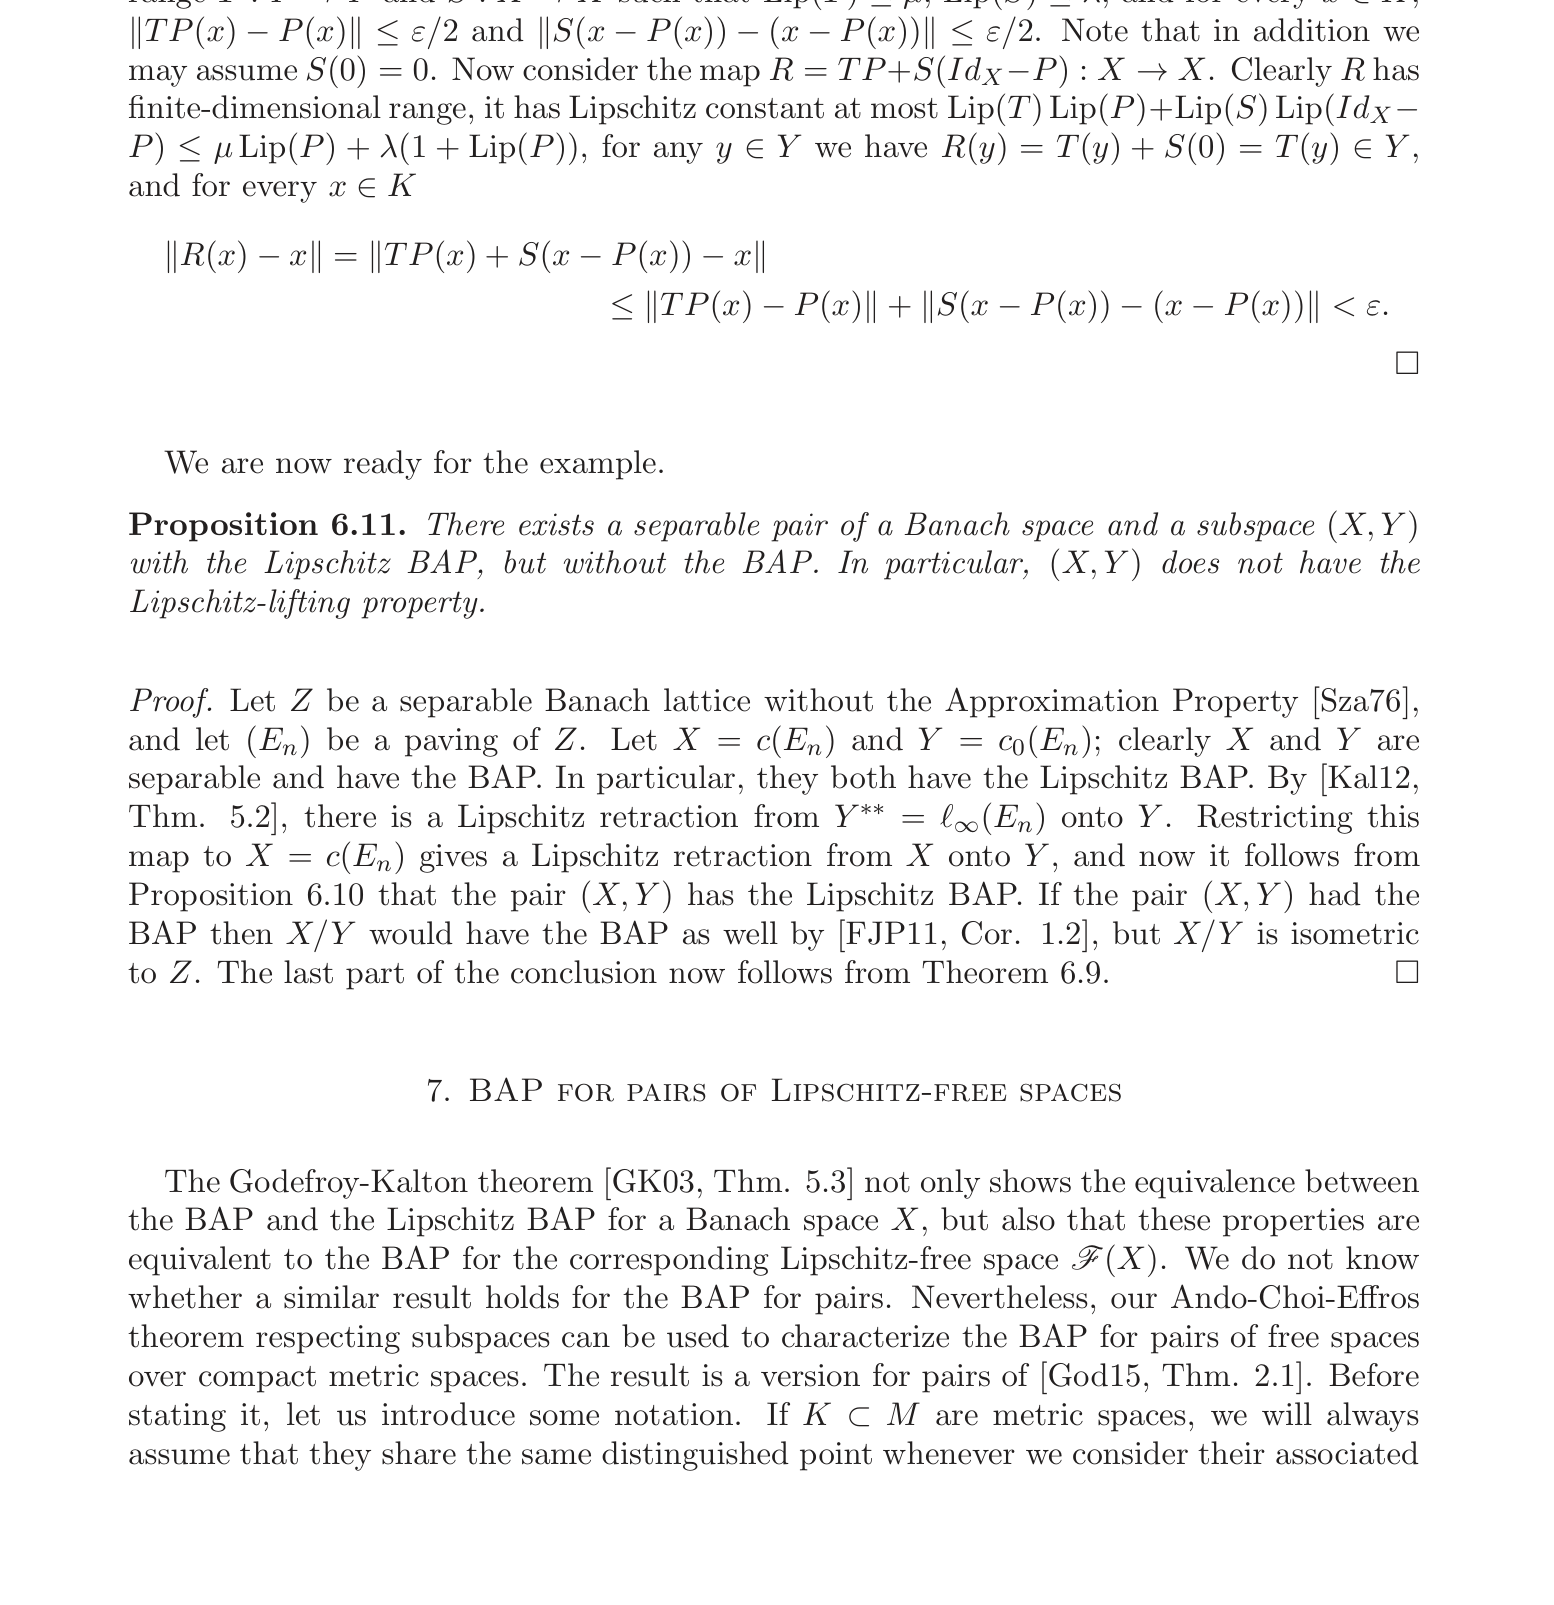
\includegraphics[width=0.96\textwidth]{figures/open_problem_and_example_crop.png}
\end{center}

\section*{Proof Intuition}

The source's Proposition 6.11 already supplies a pair \((X,Y)\) that has too
much nonlinear approximation and too little linear approximation: it has the
Lipschitz BAP but not the BAP. The extra useful feature in the proof is a
Lipschitz retraction \(P:X\to Y\). Passing to free spaces linearizes this
retraction into a bounded projection \(\widehat P:\F(X)\to \F(Y)\). Meanwhile,
the source also notes that \(X\) itself has the BAP, so the Godefroy-Kalton
theorem gives the BAP for \(\F(X)\). A complemented subspace of a BAP space
gives a BAP pair by a direct block-diagonal approximation argument. Therefore
the free-space pair has BAP even though the original pair does not.

\section*{Definitions}

For a Banach space \(X\) and a closed subspace \(Y\), the pair \((X,Y)\) has
the BAP if there is a uniformly bounded net of finite-rank operators
\(T_i:X\to X\) converging to the identity uniformly on compact subsets of \(X\)
and satisfying \(T_i(Y)\subseteq Y\) for every \(i\).

If \(M\) is a pointed metric space, \(\F(M)\) denotes its Lipschitz-free space.
A Lipschitz map \(f:M\to N\) fixing the base point has a canonical bounded
linearization \(\widehat f:\F(M)\to\F(N)\) with
\(\widehat f(\delta_m)=\delta_{f(m)}\) and
\(\|\widehat f\|=\Lip(f)\).

\section*{A Complemented-Pair Lemma}

\begin{lemma}
Let \(E\) be a Banach space with the BAP, and let \(W\subset E\) be the range
of a bounded projection \(Q:E\to E\). Then the pair \((E,W)\) has the BAP.
\end{lemma}

\begin{proof}
Choose uniformly bounded finite-rank operators \(A_i:E\to E\) converging to
\(\Id_E\) uniformly on compact subsets. Put
\[
 R_i = Q A_i Q + (\Id-Q)A_i(\Id-Q).
\]
Each \(R_i\) has finite rank and the norms are uniformly bounded. If
\(w\in W\), then \(Qw=w\) and \((\Id-Q)w=0\), so
\[
 R_iw=QA_iw\in W.
\]
Finally, every \(x\in E\) decomposes as \(x=Qx+(\Id-Q)x\), and
\[
 R_ix
 =Q A_i(Qx)+(\Id-Q)A_i((\Id-Q)x)
 \longrightarrow Qx+(\Id-Q)x=x
\]
uniformly on compact sets, because \(A_i\to\Id_E\) uniformly on compact sets
and \(Q,\Id-Q\) are bounded.
\end{proof}

\section*{Counterexample}

\begin{theorem}
There is a separable Banach-space pair \((X,Y)\) such that
\((\F(X),\F(Y))\) has the BAP, but \((X,Y)\) does not have the BAP.
\end{theorem}

\begin{proof}
Use the pair constructed in Proposition 6.11 of the source paper. Namely, let
\(Z\) be a separable Banach lattice without the approximation property, let
\((E_n)\) be a paving of \(Z\), and set
\[
 X=c(E_n),\qquad Y=c_0(E_n).
\]
The source proves that \((X,Y)\) has the Lipschitz BAP but not the BAP. It also
records two further facts from the construction: \(X\) and \(Y\) have the BAP
individually, and there is a Lipschitz retraction \(P:X\to Y\).

Since \(X\) has the BAP, the Godefroy-Kalton theorem gives the BAP for
\(\F(X)\). Since \(P\) is a Lipschitz retraction fixing \(Y\), its
linearization
\[
 \widehat P:\F(X)\to\F(Y)
\]
is a bounded projection: it maps \(\F(X)\) into \(\F(Y)\), and it restricts to
the identity on \(\F(Y)\). Applying the complemented-pair lemma to
\(E=\F(X)\), \(W=\F(Y)\), and \(Q=\widehat P\), we get that
\((\F(X),\F(Y))\) has the BAP.

Thus \((\F(X),\F(Y))\) has BAP while \((X,Y)\) does not.
\end{proof}

\section*{Scope and Limitations}

The result disproves the implication from BAP of the free-space Banach pair to
BAP of the original Banach pair. It does not contradict the source paper's
positive characterizations of BAP for \((\F(M),\F(K))\) over compact or
separable metric pairs, and it does not settle every possible formulation of a
``similar result'' for arbitrary metric pairs.

\section*{Novelty Check}

The run indexes were searched for arXiv:1702.04774, the title,
Ando-Choi-Effros lifting, BAP for pairs, Lipschitz-free spaces, and related
phrases. No exact prior packet for this source question was found. External
web searches on 2026-06-20 for phrases such as
``BAP for pairs'' with ``Lipschitz-free spaces'', ``F(X), F(Y)'' with
``BAP'' and ``pair'', and ``free-space pair'' with ``without the BAP'' returned
the source paper or no direct answer.

\section*{References}

\begin{enumerate}
\item J. A. Chavez-Dominguez, arXiv:1702.04774, 2017.
\item G. Godefroy and N. J. Kalton,
\emph{Lipschitz-free Banach spaces},
Studia Math. 159 (2003), 121--141.
\end{enumerate}

\section*{Human Review Recommendation}

The main review point is interpretive: confirm that the source's phrase
``similar result'' includes the natural Banach-pair implication
\((\F(X),\F(Y))\) BAP \(\Rightarrow (X,Y)\) BAP. Under that reading, the
counterexample is complete.

\end{document}
